%ITY - Projekt 5
%Autor: Matej Keznikl
%Fakulta: Fakulta informačných technológií VUT v Brne (FIT VUT)

\documentclass[15pt]{beamer}
\usepackage[utf8]{inputenc}
\usepackage[T1]{fontenc}
\usepackage[slovak]{babel}
\usepackage{algorithm2e}
\usepackage{tikz}
\usepackage{color}
\definecolor{My_Blue}{HTML}{1b4eb3}
\usetheme{Madrid}
\usecolortheme{whale}

\AtBeginSection[]
{
  \begin{frame}
    \frametitle{Prehľad}
    \tableofcontents[currentsection]
  \end{frame}
}

\title[Dijktrov algoritmus]{Dijktrov algoritmus}
\author{Matej Keznikl}
\institute[VUT FIT]{Fakulta informačních technologií\\Vysoké učení technické v~Brně}
\date{\today}

\begin{document}

\frame{\titlepage}

\section{Úvod do grafových algoritmov}
\begin{frame}{Definícia}
	\subsection{Definícia}
	\begin{block}{Definícia}
		Graf $G$ sa skladá z množiny vrcholov $V$ a množiny hrán $E$, pričom každá hrana spája dva rôzne vrcholy. Graf sa môže vyjadriť ako dvojica $G = (V,E)$.
	\end{block}
	\subsection{Typy grafov}
	\begin{block}{Typy grafov}
		\begin{itemize}
			\item Neorientovaný graf
			\item Orientovaný graf
			\item Úplný graf
			\item Vážený graf
			\item Strom
			\item Mriežka
		\end{itemize}
	\end{block}
\end{frame}

\section{Popis Dijkstrovho algoritmu}
\begin{frame}{Popis Dijkstrovho algoritmu}
	\subsection{Princíp}
	\begin{block}{Princíp Dijkstrovho algoritmu}
		Nech $G=(V,E)$ je orientovaný graf s nezápornými ohodnoteniami hrán, kde $V$ predstavuje množinu vrcholov a $E$ predstavuje množinu hrán s váhami $w: E \rightarrow \mathbb{R}^+_0$. Nech $s \in V$ je začiatočný vrchol. Dijkstrov algoritmus nájde najkratšiu cestu z $s$ do každého iného vrcholu v $G$. Začína s prázdnu množinou $S$ a inicializuje vzdialenosť $dist[v]$ pre každý vrchol $v \in V$ na nekonečno, okrem $s$, pre ktorý $dist[s]=0$. Ďalej opakuje nasledovné kroky, kým $S$ neobsahuje všetky vrcholy z $V$:
		\begin{enumerate}
			\item Zvoľ vrchol $u \in V$ s najmenšou hodnotou $dist[u]$ a pridaj ho do množiny $S$.
			\item Pre každú hranu $(u,v)$ vychádzajúcu z vrcholu $u$, ak $dist[u] + w(u,v) < dist[v]$, aktualizuj hodnotu $dist[v]$ na $dist[u] + w(u,v)$.
			      			      			      
		\end{enumerate}
	\end{block}
\end{frame}

\begin{frame}{Popis Dijkstrovho algoritmu}
	\begin{block}{Zložitosť}
		\subsection{Zložitosť}
		Časová zložitosť Dijkstrovho algoritmu sa dá zapísať v O-notácii ako $O((|E|+|V|)\log |V|)$, kde $|E|$ je počet hrán a $|V|$ je počet vrcholov grafu.
				
		Táto zložitosť je spôsobená tým, že Dijkstrov algoritmus prehľadáva všetky vrcholy v grafe a pre každý z nich aktualizuje vzdialenosť od počiatočného vrcholu. To znamená, že algoritmus prejde každú hranu v grafe aspoň raz. Ak by sme to zhrnuli, časová zložitosť prehľadávania grafu bez aktualizácie by bola $O(|E|+|V|)$.
	\end{block}
\end{frame}

\begin{frame}{Pseudokód Dijkstrovho algoritmu}
	\subsection{Pseudokód}
	\begin{algorithm}[H]
		\SetAlgoLined
		\KwIn{Graf $G$, začiatočný vrchol $s$}
		\KwOut{Najkratšie cesty z $s$ do každého vrcholu}
		Inicializuj vzdialenosti $\mathrm{dist}[s] = 0$ a $\mathrm{dist}[v] = \infty$ pre každý iný vrchol $v$ v grafe $G$, Inicializuj prázdnu množinu $S$;\newline
		Inicializuj frontu $Q$ obsahujúcu všetky vrcholy v grafe $G$; \newline
		\While{$Q$ nie je prázdna}
		{
			Nájdi vrchol $u$ v $Q$ s najmenšou hodnotou $\mathrm{dist}[u]$;\newline
			Odober vrchol $u$ z $Q$; \newline
			Pridaj vrchol $u$ do $S$; \newline
			\For{každý susedný vrchol $v$ vrcholu $u$}{
				\If{$\mathrm{dist}[u] + w(u,v) < \mathrm{dist}[v]$}
				{
					$\mathrm{dist}[v] = \mathrm{dist}[u] + w(u,v)$;
				}
			}
		}
	\end{algorithm}
	Kde $w(u,v)$ označuje váhu hrany medzi vrcholmi $u$ a $v$.
\end{frame}

\section{Použitie}
\begin{frame}{Ilustračný príklad}
	\subsection{Ilustračný príklad}
	Ukážka behu Dijkstrového algoritmu medzi vrcholmi u,v v nasledujúcom grafe, pričom pre každý vrchol zakreslíme jeho okamžitú dočasnú vzdialenosť vzdial[x]. (Tj. spracované vrcholy budeme
	značiť krúžkom a hrany plnou čiarou.)
	\begin{figure}
		\centering
		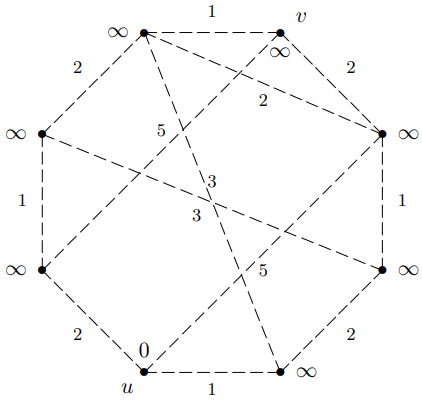
\includegraphics[width=0.48\textwidth]{imgs/dijkstra1.png}
		\label{fig:dijkstra1}
	\end{figure}
\end{frame}

\begin{frame}{Ilustračný príklad}
	\begin{figure}
		\centering
		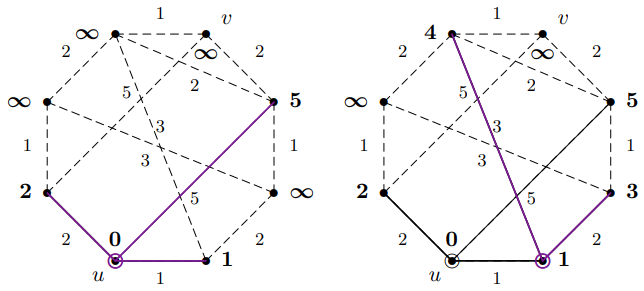
\includegraphics{imgs/dijkstra2.png}
		\caption{Krok č.1 a č.2 Dijktrového algoritmu}
		\label{fig:dijkstra2}
	\end{figure}
\end{frame}

\begin{frame}{Ilustračný príklad}
	\begin{figure}
		\centering
		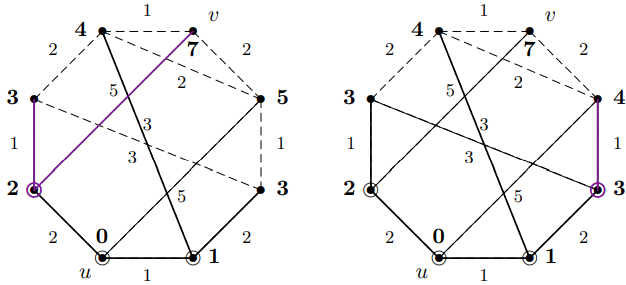
\includegraphics{imgs/dijkstra3.png}
		\caption{Krok č.3 a č.4 Dijktrového algoritmu}
		\label{fig:dijkstra3}
	\end{figure}
\end{frame}

\begin{frame}{Ilustračný príklad}
	\begin{figure}
		\centering
		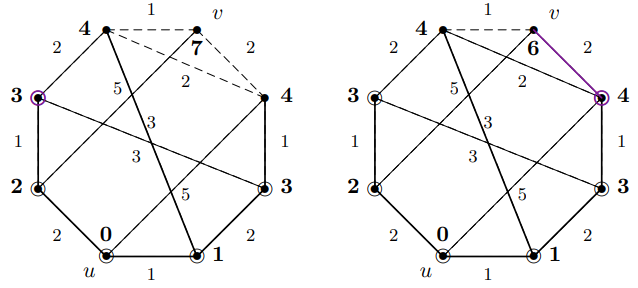
\includegraphics{imgs/dijkstra4.png}
		\caption{Krok č.5 a č.6 Dijktrového algoritmu}
		\label{fig:dijkstra4}
	\end{figure}
\end{frame}

\begin{frame}{Ilustračný príklad}
	\begin{figure}
		\centering
		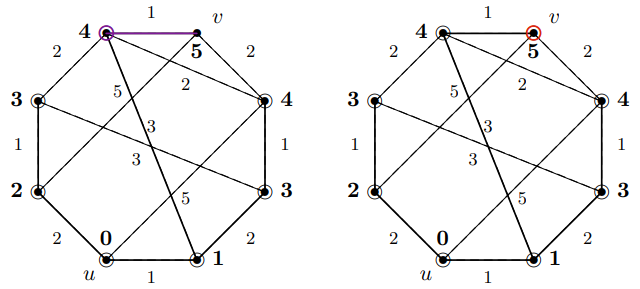
\includegraphics{imgs/dijkstra5.png}
		\caption{Krok č.7 a č.8 Dijktrového algoritmu}
		\label{fig:dijkstra5}
	\end{figure}
\end{frame}

\begin{frame}{Príklady použitia}
	\subsection{Príklady použitia}
	\begin{itemize}
		\item Dopravná sieť - najrýchlejšia cesta alebo cesta s najmenším počtom prestupov.
		\item Telekomunikačné siete - hľadanie najkratšej cesty medzi dvoma bodmi v sieti
		\item GPS navigácia - vypočítanie najkratšej cesty medzi dvomi bodmi na mape
		\item Finančný manažment - hľadanie najefektívnejšej cesty ako investovať peniaze
		\item Biológia - hľadanie najkratšej cesty medzi dvoma bodmi v DNA reťazcoch alebo v proteínových sieťach
	\end{itemize}
\end{frame}

\section{Zhrnutie}
\begin{frame}{Zhrnutie}
		
	\begin{block}{Výhody Dijstrovho algoritmu}
		\begin{itemize}
			\item Dijkstrov algoritmus je jednoduchý na pochopenie a implementáciu.
			\item Môže byť použitý na riešenie širokej škály problémov týkajúcich sa najkratšej cesty v grafe.
			\item Algoritmus je optimálny, t.j. vždy nájde najkratšiu cestu medzi dvoma bodmi.
			\item Prehľadná a intuitívna vizualizácia - napríklad Dijkstrov algoritmus môže byť jednoducho vizualizovaný ako "vlna" šíriaca sa cez graf.
		\end{itemize}
	\end{block}
		
	\begin{block}{Nevýhody Dijstrovho algoritmu}
		\begin{itemize}
			\item Dijkstrov algoritmus má exponenciálnu časovú zložitosť, čo znamená, že pre veľké grafy môže byť príliš pomalý.
			\item Algoritmus neberie do úvahy negatívne váhy hrán. Preto, ak sú v grafe negatívne hrany, môže byť použitie Dijkstrovho algoritmu nevhodné.
		\end{itemize}
	\end{block}
\end{frame}

\begin{frame}{Použité zdroje}
	\url{https://www.umat.fekt.vut.cz/~hlinena/IDM/SadyUloh/grafy.pdf}
\end{frame}

\begin{frame}{}
	\centering \Huge \emph{Ďakujem za pozornosť!}
\end{frame}
\end{document}